\documentclass{article}

\usepackage[bookmarksnumbered, colorlinks, plainpages]{hyperref}
\usepackage{fancyhdr}
\usepackage{extramarks}
\usepackage{amsmath}
\usepackage{amsthm}
\usepackage{amsfonts}
\usepackage{tikz}
\usepackage[plain]{algorithm}
\usepackage{algpseudocode}
\usepackage{graphicx}
\usepackage{tabularx}

\graphicspath{ {./img/} }
\usetikzlibrary{automata, positioning}

%
% Basic Document Settings
%

\topmargin=-0.45in
\evensidemargin=0in
\oddsidemargin=0in
\textwidth=6.5in
\textheight=9.0in
\headsep=0.25in

\linespread{1.1}

\pagestyle{fancy}
\lhead{\hmwkAuthorName}
\chead{\hmwkClass\ (\hmwkClassInstructor\ \hmwkClassTime): \hmwkTitle}
\rhead{\firstxmark}
\lfoot{\lastxmark}
\cfoot{\thepage}

\renewcommand\headrulewidth{0.4pt}
\renewcommand\footrulewidth{0.4pt}

\setlength\parindent{0pt}

%
% Create Problem Sections
%

\newcommand{\enterProblemHeader}[1]{
    \nobreak\extramarks{}{Problem \arabic{#1} continued on next page\ldots}\nobreak{}
    \nobreak\extramarks{Problem \arabic{#1} (continued)}{Problem \arabic{#1}
    continued on next page\ldots}\nobreak{}
}

\newcommand{\exitProblemHeader}[1]{
    \nobreak\extramarks{Problem \arabic{#1} (continued)}{Problem \arabic{#1}
    continued on next page\ldots}\nobreak{}
    \stepcounter{#1}
    \nobreak\extramarks{Problem \arabic{#1}}{}\nobreak{}
}

\setcounter{secnumdepth}{0}
\newcounter{partCounter}
\newcounter{homeworkProblemCounter}
\setcounter{homeworkProblemCounter}{1}
\nobreak\extramarks{Problem \arabic{homeworkProblemCounter}}{}\nobreak{}

%
% Homework Problem Environment
%

\newenvironment{homeworkProblem}[1]{
    \section{Problem \arabic{homeworkProblemCounter}{#1}}
    \setcounter{partCounter}{1}
    \enterProblemHeader{homeworkProblemCounter}
}{
    \exitProblemHeader{homeworkProblemCounter}
}

%
% Homework Details
%   - Title
%   - Due date
%   - Class
%   - Section/Time
%   - Instructor
%   - Author
%

\newcommand{\hmwkTitle}{Homework\ 6}
\newcommand{\hmwkDueDate}{April 5, 2024}
\newcommand{\hmwkClass}{CS 362}
\newcommand{\hmwkClassTime}{11:00am}
\newcommand{\hmwkClassInstructor}{Professor Troy}
\newcommand{\hmwkAuthorName}{\textbf{Ryan Magdaleno}}
\newcommand{\hwline}{\begin{center}\line(1,0){358px}\end{center}}

%
% Title Page
%

\title{
    \vspace{2in}
    \textmd{\textbf{\hmwkClass:\ \hmwkTitle}}\\
    \normalsize\vspace{0.1in}\small{Due\ on\ \hmwkDueDate\ at 11:59pm}\\
    \vspace{0.1in}\large{\textit{\hmwkClassInstructor\ \hmwkClassTime}}
    \vspace{3in}
}

\author{\hmwkAuthorName\\\href{mailto:rmagd2@uic.edu}{rmagd2@uic.edu}}
\date{}

\renewcommand{\part}[1]{\textbf{\large Part \Alph{partCounter}}
\stepcounter{partCounter}\\}
%
% Various Helper Commands
%

% Useful for algorithms
\newcommand{\alg}[1]{\textsc{\bfseries \footnotesize #1}}

% For derivatives
\newcommand{\deriv}[1]{\frac{\mathrm{d}}{\mathrm{d}x} (#1)}

% For partial derivatives
\newcommand{\pderiv}[2]{\frac{\partial}{\partial #1} (#2)}

% Integral ds
\newcommand{\dx}{\mathrm{d}x}
\newcommand{\D}[1]{\mathrm{d}#1}

% Image insertion
\newcommand{\img}[2]{\begin{center}\includegraphics[scale=#1]{#2}\end{center}}

% Alias for the Solution section header
\newcommand{\solution}{\textbf{\large Solution}\\}

% Probability commands: Expectation, Variance, Covariance, Bias
\newcommand{\E}{\mathrm{E}}
\newcommand{\Var}{\mathrm{Var}}
\newcommand{\Cov}{\mathrm{Cov}}
\newcommand{\Bias}{\mathrm{Bias}}

\begin{document}

\maketitle

\pagebreak

%%%%%%%%%%%%%%%%%%%%%%%%%%%%%%%%%%%%%%%%%%%%%%%%%%%%%%%%%%%%%%%%%%%%%%%%%%%%%%%%%%%%%%%%%

\begin{homeworkProblem}{}
    Consider the following Finite State Machine. Start State: S0 \\
    Output value is under the line below the State number. 
    \img{0.3}{1.png}
\end{homeworkProblem}
\hwline\solution
\begin{enumerate}
    \item\vspace{-5pt}
    Is the above FSM a Moore machine or a Mealy Machine? \\
    Mealy Machine.
    \hwline
    \item\vspace{-5pt}
    What is output by the above FSM for the: \\
    Input:\\1 0 1 1 0 0 0 1 0 0 1 1 \\
    Output:\\ 0 1 0 1 0 1 0 1 1 0 1 1 0
    \hwline
    \item\vspace{-5pt}
    Create the truth table to the above FSM. Encode the states using 2 bit binary 
    values:\\
    S0 $\rightarrow$ 0 0, S1 $\rightarrow$ 0 1, S2 $\rightarrow$ 1 0, S3 $\rightarrow$ 1 1
    \\
    \begin{tabularx}{0.9\textwidth} { 
        | >{\centering\arraybackslash}X 
        | >{\centering\arraybackslash}X 
        | >{\centering\arraybackslash}X 
        | >{\centering\arraybackslash}X 
        | >{\centering\arraybackslash}X 
        | >{\centering\arraybackslash}X | }
        \hline $p1$ & $p0$ & $b$ & y & $n1$ & $n0$ \\
        \hline 0 & 0 & 0 & 0 & 1 & 1 \\
        \hline 0 & 0 & 1 & 0 & 0 & 1 \\
        \hline 0 & 1 & 0 & 1 & 0 & 0 \\
        \hline 0 & 1 & 1 & 1 & 1 & 0 \\
        \hline 1 & 0 & 0 & 0 & 0 & 1 \\
        \hline 1 & 0 & 1 & 0 & 1 & 0 \\
        \hline 1 & 1 & 0 & 1 & 1 & 0 \\
        \hline 1 & 1 & 1 & 1 & 0 & 1 \\
        \hline
    \end{tabularx}
    \hwline
    \pagebreak
    \item\vspace{-5pt}
    Write out the simplified expressions for the next state and output values. You can 
    use K-maps or boolean algebra to determine simplified expression.
    \begin{align*}
        n0 &= p1p0b + p1p0'b' + p1'p0'b + p1'p0'b' \\
        n1 &= p1'p0'b' + p1p0'b + p1'p0b + p1p0b'
    \end{align*}
    \img{0.2}{n0.png}
    $$n0 = p1'p0' + p1p0b + b'p0'$$
    \img{0.2}{n1.png}
    $$n1 = p1'p0'b' + p1p0b' + p1'p0b + p1p0'b$$
    \img{0.2}{y.png}
    $$y = p0$$
    \hwline
    \pagebreak
    \item\vspace{-5pt}
    Draw the circuit diagram for the Finite State Machine. Use the format as shown in 
    class and in the zyBooks (and in Q3 below) that contain a state register and a 
    combination logic block.
    \img{0.25}{1e.png}
    \hwline
\end{enumerate}
\pagebreak

%%%%%%%%%%%%%%%%%%%%%%%%%%%%%%%%%%%%%%%%%%%%%%%%%%%%%%%%%%%%%%%%%%%%%%%%%%%%%%%%%%%%%%%%%

\begin{homeworkProblem}{}
    Consider the following Finite State Machine. Start State: S0. \\
    Inputs are listed before the slash on each transition. \\
    Outputs are listed after the slash on each transistion.
    \img{0.3}{2.png}
    \hwline\solution
    \begin{enumerate}
        \item\vspace{-5pt}
        Is the above FSM a Moore machine or a Mealy machine? \\
        Mealy Machine
        \hwline
        \item\vspace{-5pt}
        What is output by the above FSM for: \\
        Input: 1 0 1 1 0 0 0 1 0 0 1 1 \\
        Output: 0 1 0 1 1 0 0 0 1 0 0 1
        \hwline
        \item\vspace{-5pt}
        Create the truth table to the above FSM. Encode the states using 2 bit binary 
        values: \\
        S0 $\rightarrow$ 0 0, S1 $\rightarrow$ 0 1, S2 $\rightarrow$ 1 0
        \\
        \begin{tabularx}{0.9\textwidth} { 
            | >{\centering\arraybackslash}X 
            | >{\centering\arraybackslash}X 
            | >{\centering\arraybackslash}X 
            | >{\centering\arraybackslash}X 
            | >{\centering\arraybackslash}X 
            | >{\centering\arraybackslash}X | }
            \hline $p1$ & $p0$ & $b$ & y & $n1$ & $n0$ \\
            \hline 0 & 0 & 0 & 0 & 1 & 0 \\
            \hline 0 & 0 & 1 & 0 & 0 & 1 \\
            \hline 0 & 1 & 0 & 1 & 1 & 0 \\
            \hline 0 & 1 & 1 & 1 & 0 & 1 \\
            \hline 1 & 0 & 0 & 0 & 1 & 0 \\
            \hline 1 & 0 & 1 & 0 & 0 & 1 \\
            \hline 1 & 1 & 0 & $x$ & $x$ & $x$ \\
            \hline 1 & 1 & 1 & $x$ & $x$ & $x$ \\
            \hline
        \end{tabularx}
        \hwline
        \pagebreak
        \item\vspace{-5pt}
        Write out the simplified expressions for the next state and output values. You 
        can use K-maps or boolean algebra to determine simplified expressions.
        \img{0.2}{nn0.png}
        $$n0 = b$$
        \img{0.2}{nn1.png}
        $$n1 = b'$$
        \img{0.2}{yy.png}
        $$y = b$$
        \hwline
        \pagebreak
        \item\vspace{-5pt}
        Draw the circuit diagram for the Finite State Machine. Use the format as shown in 
        class and in the zyBooks (and in Q3 below) that contain a state register and a 
        combination logic block.
        \img{0.3}{2c.png}
        \hwline
    \end{enumerate}
\end{homeworkProblem}
\pagebreak

%%%%%%%%%%%%%%%%%%%%%%%%%%%%%%%%%%%%%%%%%%%%%%%%%%%%%%%%%%%%%%%%%%%%%%%%%%%%%%%%%%%%%%%%%

\begin{homeworkProblem}{}
    Consider the following circuit:
    \img{0.3}{3.png}
    \hwline\solution
    \begin{enumerate}
        \item\vspace{-5pt}
        Write the equations for the for the next state and output values from the above 
        controller.
        \img{0.3}{3a.png}
        \begin{align*}
            n0 &= p1'a \\
            n1 &= p1a+p0a \\
            y  &= A'\cdot(p0+p1)
        \end{align*}
        \hwline
        \pagebreak
        \item\vspace{-5pt}
        Create the truth table for the above circuit: \\
        \begin{tabularx}{0.9\textwidth} { 
            | >{\centering\arraybackslash}X 
            | >{\centering\arraybackslash}X 
            | >{\centering\arraybackslash}X 
            | >{\centering\arraybackslash}X 
            | >{\centering\arraybackslash}X 
            | >{\centering\arraybackslash}X | }
            \hline $p1$ & $p0$ & $A$ & $Y$ & $n1$ & $n0$ \\
            \hline 0 & 0 & 0 & 0 & 0 & 0 \\
            \hline 0 & 0 & 1 & 0 & 0 & 1 \\
            \hline 0 & 1 & 0 & 1 & 0 & 0 \\
            \hline 0 & 1 & 1 & 0 & 1 & 1 \\
            \hline 1 & 0 & 0 & 1 & 0 & 0 \\
            \hline 1 & 0 & 1 & 0 & 1 & 0 \\
            \hline 1 & 1 & 0 & 1 & 0 & 0 \\
            \hline 1 & 1 & l & 0 & 1 & 0 \\
            \hline
        \end{tabularx}
        \hwline
        \item\vspace{-5pt}
        What information needed for drawing a Finite State Machine is not included in the 
        Truth Table and will need to be assumed? \\
        We need to assume some start state, I will divide the truth table
        into four states, $S_0$ will be the first two rows in the table, this will
        be our start state.
        \hwline
        \item\vspace{-5pt}
        Draw the Finite State Machine that is represented by the circuit:
        \begin{center}
            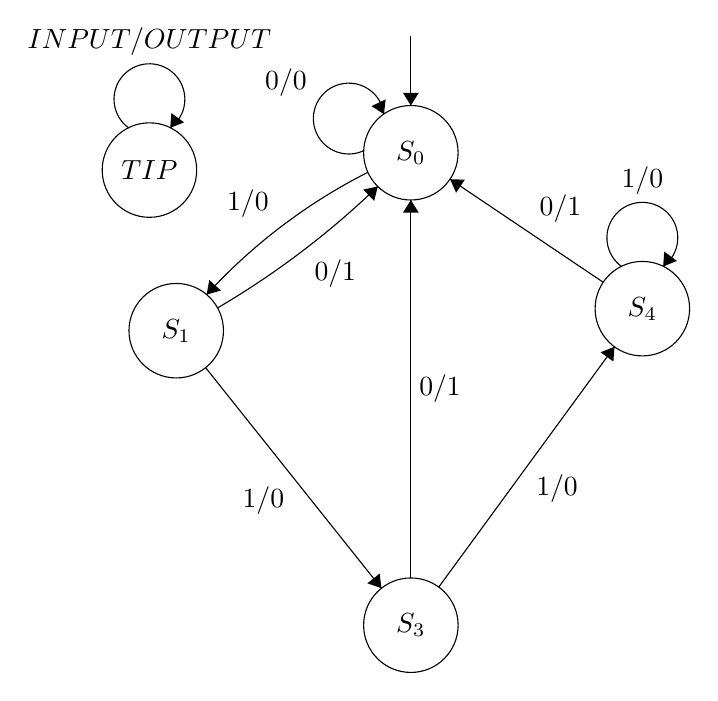
\begin{tikzpicture}[scale=0.2]
            \tikzstyle{every node}+=[inner sep=0pt]
            \draw [black] (35.2,-15.4) circle (3);
            \draw (35.2,-15.4) node {$S_0$};
            \draw [black] (20.3,-26.7) circle (3);
            \draw (20.3,-26.7) node {$S_1$};
            \draw [black] (35.2,-45.4) circle (3);
            \draw (35.2,-45.4) node {$S_3$};
            \draw [black] (49.9,-25.3) circle (3);
            \draw (49.9,-25.3) node {$S_4$};
            \draw [black] (18.6,-16.5) circle (3);
            \draw (18.6,-16.5) node {$TIP$};
            \draw [black] (35.2,-8) -- (35.2,-12.4);
            \fill [black] (35.2,-12.4) -- (35.7,-11.6) -- (34.7,-11.6);
            \draw [black] (32.215,-15.265) arc (295.14721:7.14721:2.25);
            \draw (28.62,-10.95) node [left] {$0/0$};
            \fill [black] (33.49,-12.95) -- (33.6,-12.01) -- (32.7,-12.44);
            \draw [black] (22.232,-24.406) arc (137.50543:116.84715:35.832);
            \fill [black] (22.23,-24.41) -- (23.14,-24.15) -- (22.4,-23.48);
            \draw (24.85,-19.56) node [above] {$1/0$};
            \draw [black] (33.099,-17.54) arc (-46.06004:-59.58738:54.191);
            \fill [black] (33.1,-17.54) -- (32.18,-17.74) -- (32.87,-18.46);
            \draw (30.4,-22.19) node [below] {$0/1$};
            \draw [black] (35.2,-42.4) -- (35.2,-18.4);
            \fill [black] (35.2,-18.4) -- (34.7,-19.2) -- (35.7,-19.2);
            \draw (35.7,-30.4) node [right] {$0/1$};
            \draw [black] (47.41,-23.62) -- (37.69,-17.08);
            \fill [black] (37.69,-17.08) -- (38.07,-17.94) -- (38.63,-17.11);
            \draw (44.7,-19.85) node [above] {$0/1$};
            \draw [black] (48.577,-22.62) arc (234:-54:2.25);
            \draw (49.9,-18.05) node [above] {$1/0$};
            \fill [black] (51.22,-22.62) -- (52.1,-22.27) -- (51.29,-21.68);
            \draw [black] (36.97,-42.98) -- (48.13,-27.72);
            \fill [black] (48.13,-27.72) -- (47.25,-28.07) -- (48.06,-28.66);
            \draw (43.13,-36.74) node [right] {$1/0$};
            \draw [black] (22.17,-29.05) -- (33.33,-43.05);
            \fill [black] (33.33,-43.05) -- (33.22,-42.12) -- (32.44,-42.74);
            \draw (27.19,-37.47) node [left] {$1/0$};
            \draw [black] (17.277,-13.82) arc (234:-54:2.25);
            \draw (18.6,-9.25) node [above] {$INPUT/OUTPUT$};
            \fill [black] (19.92,-13.82) -- (20.8,-13.47) -- (19.99,-12.88);
            \end{tikzpicture}
        \end{center}
        \hwline
        \item\vspace{-5pt}
        Is the Finite State Machine a Moore machine or a Mealy machine? \\
        Mealy machine.
        \hwline
        \item\vspace{-5pt}
        What is output by the above FSM for: \\
        Input: 1 0 1 1 0 0 0 1 0 0 1 1\\
        Output: 0 1 0 0 1 0 0 0 1 0 0 0
        \hwline
    \end{enumerate}
\end{homeworkProblem}
\end{document}